\documentclass[10pt,a4paper]{article}
\usepackage[margin=18mm]{geometry}
\usepackage{amsmath,amssymb,graphicx,xcolor,booktabs}
\usepackage[colorlinks=true,urlcolor=blue]{hyperref}
\usepackage[font=small,labelfont=bf]{caption}
\setlength{\parindent}{0pt}
\setlength{\parskip}{5pt}
\graphicspath{{figures/}}
\begin{document}
\begin{center}
{\Large\bfseries Fourth-order interpolation: production validation}\\[4pt]
{\small Branch \texttt{atom-fourier-interpolation}; implementation \texttt{e98eafcc}}
\end{center}

\textbf{Verdict.} The fourth-order interpolation passes the finite-range
polynomial benchmark. No defect was found in its resolved-support operator.
A separate bug in \texttt{ignore\_v3} was found and fixed: it previously
removed only one direction of the cubic coupling. The combined regression
suite passes all 56 tests, including 16 new deterministic production tests.

\textbf{Controlled physical model.}
Let $x_n$ be a mass-weighted molecular internal displacement,
$s_n(h)=\sum_r h_r x_{n+r}$, and $\omega_q^2=1+0.8\cos(2\pi q)$.
In units $\hbar=m=a=1$, the potential is
\begin{equation}
 V=\tfrac12 x^T Kx+
 \frac{g}{6}\sum_n(s_n^3-3C_hs_n)
 +\sum_{d,n}\frac{\lambda_d}{24}
 (s_{d,n}^4-6C_ds_{d,n}^2+3C_d^2).
\end{equation}
The cubic coefficients are $(g,h)=(0.08,[1,0.35])$; the quartics are
$(\lambda,h)=(0.12,[1,0.37,-0.29,0.21])$ and $(0.04,[1,-0.23])$.
Positive quartics bound the potential below. The cutoff is three cells, and
the first quartic couples \emph{four distinct cells}. At $Q=0$, the optical
frequency $\sqrt{1.8}$ lies above the two-phonon threshold $2\sqrt{0.2}$.

$C_h=\langle s(h)^2\rangle$ is fixed from the prescribed coarse Gaussian.
The counterterms cancel its mean anharmonic force and curvature.
\textbf{Neither the potential nor the harmonic reference is re-minimized
on the fine mesh.} Degree-seven Gaussian quadrature exactly integrates the
polynomial force estimator, eliminating Monte Carlo uncertainty.

\begin{figure}[ht]
\centering
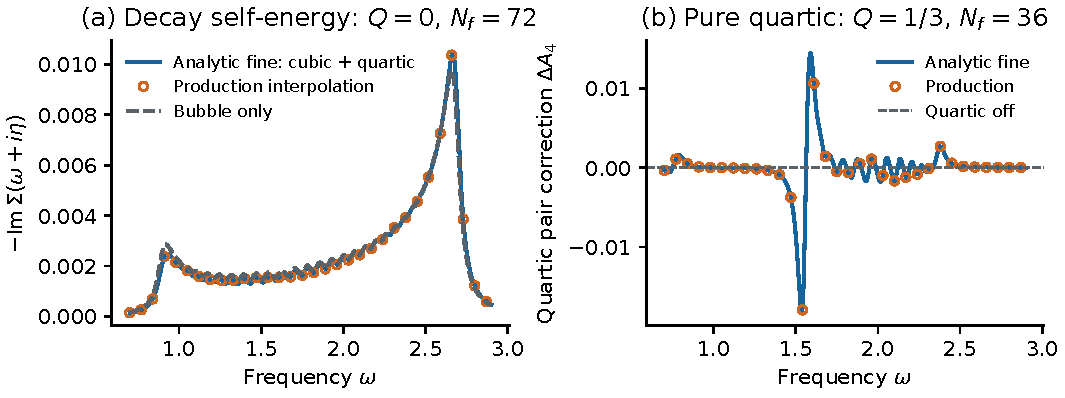
\includegraphics[width=\linewidth]{response.pdf}
\caption{Actual production fold--Julia contraction--reconstruction, compared
with analytic fine-mesh derivatives of the same potential. (a) Imaginary
self-energy, with and without quartic resummation, at $T=0$.
(b) Quartic change in the pair response, with cubic coupling disabled, at $k_BT=0.3$:
the difference of $-\operatorname{Im}\operatorname{Tr}(z^2I+L_{\rm pair})^{-1}/(\pi d)$
with and without the quartic vertex; $d$ is the pair-block dimension. Both use $N_c=9$ and
$z=\omega+0.04i$. Open markers overlay the analytic curves; dashed curves
show that the quartic contribution is measurable. This is a regulated
finite-mesh response, not an extrapolated thermodynamic lifetime.}
\end{figure}

\newpage
\textbf{Why the test establishes interpolation accuracy.}
The independent reference uses analytic vertices $v=\Phi^{(3)}/\sqrt{N_f}$
and $W=\Phi^{(4)}/N_f$, with the full ordered-pair convention:
\begin{equation}
 \Sigma(z)=v^\dagger[I-\Lambda(z)W]^{-1}\Lambda(z)v,
 \qquad G(z)=[z^2-\omega_Q^2-\Sigma(z)]^{-1}.
\end{equation}
At fixed external $Q$, a finite-range quartic vertex is a trigonometric
polynomial in \emph{two independent internal momenta}. Production interpolates
both pair legs with normalization $N_c/N_f$. When the real-space support is
resolved by the centered coarse mesh, the tensor is reconstructed before
response inversion. The reference does not reuse that interpolation.

\begin{figure}[ht]
\centering
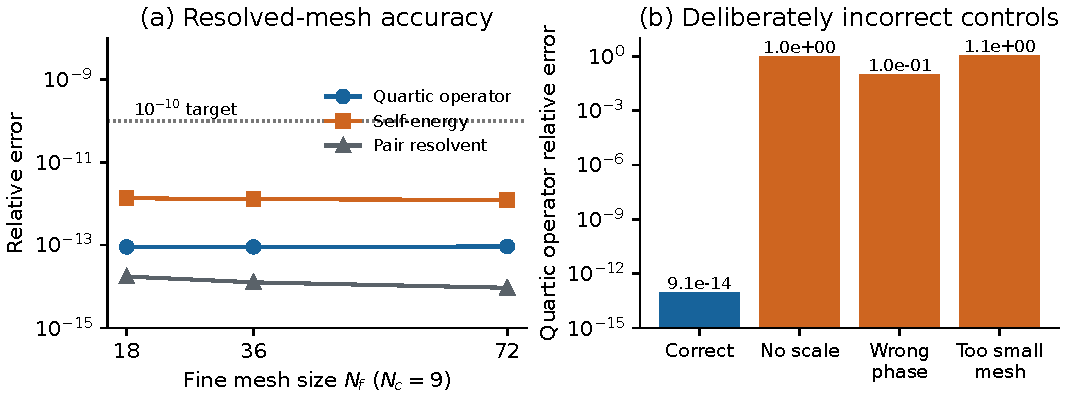
\includegraphics[width=\linewidth]{accuracy.pdf}
\caption{(a) Production versus independent analytic fine reference at
$Q=1/3$, $k_BT=0.3$, and $\eta=0.04$. Operator errors are relative Frobenius
norms after subtracting the harmonic block; self-energy and pair-resolvent
errors are maxima over 41 frequencies in $[0.3,2.8]$.
(b) Negative controls: omitting the mesh factor, conjugating the kernel
incorrectly, or using $N_c=3$ for the same three-cell interaction produces
large quartic errors. The first three bars use $9\to18$, $Q=1/3$;
the last uses $3\to18$, $Q=0$; all four controls have $T=0$.}
\end{figure}

The regression checks isolate cubic and quartic operators, bubble and
resummed self-energies, and the pure-quartic pair resolvent. They include
$9\to9/18/36/72$ and $8\to24$ meshes, nonzero $Q$, finite-temperature
sum/difference channels, unequal masses, atom rebasing, dense complex mode
mixing, and acoustic masks. Vertices and resolvents satisfy $10^{-10}$
tolerances; self-energy satisfies $10^{-8}$.

Interpolating an \emph{already computed response} is a different operation:
the response is not finite range. The separate analytic off-grid control at
$Q=1/18$ gives about $31\%$ error, even using identical fine internal
quadrature. Production currently requires external $Q$ on the coarse mesh;
this control does not claim otherwise.

\textbf{What was wrong and what was right.}
The quartic interpolation was right in these resolved-support tests.
The \texttt{ignore\_v3} switch was wrong: it removed the one-phonon-to-pair
coupling but retained the reverse coupling. Both q-space classes now remove
both directions, restoring pure-quartic isolation. This fix does not change
the usual calculation with cubic coupling enabled.

\small
\textbf{Reproduction.} From this checkout with its Python/Julia environment,
run \path{benchmarks/interpolation/make_report_figures.py}.
The plotted arrays and source hashes accompany the vector figures.
The exact test command is in the adjacent \texttt{README.md}.
Compile this file with \texttt{pdflatex} from its directory.
\end{document}
